
%----------------------------------------------------------------------------------------
%	SECTION
%----------------------------------------------------------------------------------------
\section{Heap and System Calls}
\label{sec:heap}

In the order to understand dynamic memory allocation, we need to understand how the memory of a process executing a program is handled in most operating systems. We will keep an abstract point of view for that part, since many details are operating system and
hardware dependent.

\subsection{The Process’s Memory}
Every process has its own virtual address space which is dynamically translated into physical memory  address space by the memory management unit (MMU) and the kernel. This memory space may be seen as a contiguous array of bites, like in Figure~\ref{fig:memory}. It is divided in several parts, mainly:
\begin{itemize}
\item the text part containing the code executed,
\item the data part space for constant and global variables,
\item the stack where local variables of functions called during the process execution are stored, and 
\item the program’s data created during the execution, called the \emph{heap}.
\end{itemize}

The DMA manages the heap. The heap is a continuous (in terms of virtual addresses) space of memory blocks with three bounds (see Figure~\ref{fig:memory}): 
a starting point, 
a maximum limit (managed through \code{sys/resource.h}’s functions \code{getrlimit()} and \code{setrlimit()}) and 
an end point called the break. The break marks the end of the used memory space, that is, the part of the heap that is managed by the dynamic allocation \cite{WilsonJNB95}.

\begin{figure}[htbp]
    \begin{center}
        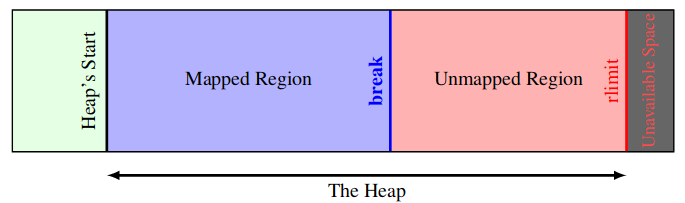
\includegraphics[width=0.8\textwidth]{figures/heap}
    \caption{Memory organization}
    \label{fig:memory}
    \end{center}
\end{figure}


\subsection{System Calls}

To manage the heap, the DMA calls low level primitives of the operating system in order to obtain the starting point of the heap and the break point position; it also needs to be able to move the break point.
For the Unix systems, these primitives are \code{brk()} and \code{sbrk()}, whose signature is:
\begin{lstlisting}[style=cstyle]
int brk(const void *addr);
void* sbrk(intptr_t incr);
\end{lstlisting}

As specified by the Unix manual, \code{brk()} and \code{sbrk()} change the location of the break point. Increasing the break point has the effect of allocating heap memory to the process; decreasing the break deallocates memory.

\code{brk()} sets the break point to the value specified by \code{addr}, when that value is reasonable, the system has enough memory, and the process does not exceed its maximum more limit.

\code{sbrk()} increments the break point by \code{incr} bytes, with the same limitations like above. Calling \code{sbrk()} with an increment of 0 can be used to find the current location of the program break.

On success, \code{brk()} returns zero. On error, \code{-1} is returned. %, and \code{errno} is set to \code{ENOMEM}.
%
On success, \code{sbrk()} returns the previous program break. (If the break was increased, then this value is a pointer to the start of the newly allocated memory). On error, \code{(void *) -1} is returned. %, and \code{errno} is set to \code{ENOMEM}.\\


\subsection{Heap Initialization}

Using these system calls, the DMA starts from a initial size of the heap and moves the break depending on the client's needs. The initial configuration of the heap region may be fixed to some \code{size} using the following code,
where the global variables \code{hit} and \code{hli} denote the start respectively the limit (first after the last) address of the memory region managed:

\begin{lstlisting}[style=cstyle]
void minit(int size) 
{ hst=sbrk(size); hli=sbrk(0); }
\end{lstlisting}

Figure~\ref{fig:init} illustrates the heap region obtained with the above code.
In this region, the DMA manages its own data and the data allocated for the process.
 
\begin{figure}[htbp]
    \begin{center}
        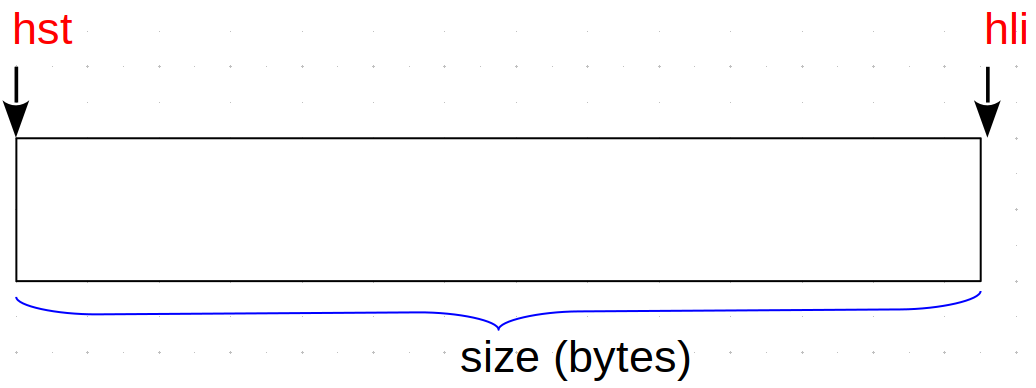
\includegraphics[width=0.6\textwidth]{figures/sbrk}
    \caption{Initial configuration of the heap}
    \label{fig:init}
    \end{center}
\end{figure}




%----------------------------------------------------------------------------------------
%	SECTION
%----------------------------------------------------------------------------------------

\section{Dynamic Memory Allocation}
\label{sec:dma}

We focus on this work on the DMA for the C language.

\subsection{User interface}

Usually, programs use the dynamic memory allocation to add a node to a data structure whose size is not known. In object oriented languages, dynamic memory allocation is used to get the memory for a new object, for example the primitive \code{new} in Java. The program may ask for memory of different sizes at different execution points.

Memory allocated may be returned whenever it is no longer needed. Memory can be returned in any order without any relation to the order in which it was allocated. 

Two functions make it possible to reserve and release dynamically an area of memory: \code{malloc()} for the reservation and \code{free()} for the liberation of previously allocated memory via \code{malloc()}.

\subsubsection{Memory allocation}
\code{malloc} is a C standard library function which is used to allocate a block of memory on the heap. The program accesses this block of memory via a pointer that \code{malloc} returns.
The function signature is:

\begin{lstlisting}[style=cstyle]
void* malloc(size_t size);
\end{lstlisting}

The only parameter to pass to malloc is \code{size}, the \emph{number of bytes} to allocate. The returned value is the address of the first byte of the allocated memory area. If the allocation could not be realized (due to lack of free memory), the return value is the \code{NULL} constant.

\subsubsection{Memory release}
When memory returned by \code{malloc()} is no longer useful, it doesn't get freed on its own. In the order to release the space allocated before, the program should explicitly use another C standard library function: \code{free()}.
The function signature is:
\begin{lstlisting}[style=cstyle]
void free(void *ptr);
\end{lstlisting}
\code{free()} releases the memory space pointed by \code{ptr}, which shall be a pointer obtained on a previous call to \code{malloc()}. If \code{ptr} has already been released, the behavior of \code{free()} is undetermined and it is considered a programming flaw. If \code{ptr} is \code{NULL}, no attempt to release takes place.


\subsubsection{Memory fragmentation}
The heap region managed by the DMA (see Figure~\ref{fig:init}) is initially considered free  and may be allocated entirely by a call to \code{malloc} of the size nearly equal to \code{size}.
However, programs are usually asking for smaller blocks, which are reserved by splitting the  heap region managed by the DMA in several \emph{chunks}. I will present the precise organization of a chunk in the next section.

What is important here is to know that a chunk stores the block of memory required by the program and some internal data used by the DMA to manage the chunk.

With this splitting in chunks, the heap region may develop ``holes'' where previously allocated memory has been returned between blocks of memory still in use.
A new request for memory might return a range of addresses out of one of the holes. But it might not use up all the hole, so further dynamic requests might be satisfied out of the original hole.

If too many small holes develop, memory is wasted because the total memory used by the holes may be large, but the holes cannot be used to satisfy dynamic requests. This situation is called \emph{memory fragmentation} \cite{Knuth73a}. 

\subsection{Properties of good allocators}
An allocator must keep tracking chunks which are in use and free.
The main goals of a good allocator are \cite{Lea12}:
\begin{itemize}
\item Maximizing compatibility: The implemented allocator must be compatible with ANSI/POSIX conventions.
\item Maximizing portability: The allocator must cover as many systems as possible.
\item Minimizing space: The allocator shouldn't waste space and track contiguous chunk to minimize fragmentation.
\item Minimizing time: The time for allocation and release of memory should be as short as possible.
\item Maximizing tunability: Optional features and behavior should be controllable by users either statically (via \code{#define} and the like) or dynamically (via control commands such as \code{mallopt}).
\item Maximizing locality: Allocate chunks of memory that are typically used together near each other. This helps minimize page and cache misses during program execution.
\item Maximizing error detection: Ensure that the use of the allocator is safe by checking the parameters received. 
Also, it does not seem possible for a general-purpose allocator to also serve as general-purpose memory error testing tool such as Purify. However, allocators should provide some means for detecting corruption due to overwriting memory, multiple frees, and so on.
\end{itemize}



%----------------------------------------------------------------------------------------
%	SECTION
%----------------------------------------------------------------------------------------

\section{Implementing an Allocator}
\label{sec:impl}
Allocators are categorized by the mechanisms they use to keep track of free chunks and to coalesce neighboring free chunks.
In what follows, I will explain step by step the design principles of a class of allocators that manages free chunks using a list.

\subsection{Chunk Information}
At the beginning of every chunk, the DMA stores extra-informations, called meta-data (see Figure~\ref{fig:chunkrep}), about
the size of the chunk, a flag to mark free chunks (free or busy), the pointer to the next or previous free chunk. 
the pointer returned by \code{malloc} is the address in the chunk after this meta-data, that we call \emph{chunk header} in the following.

\begin{figure}[htbp]
    \begin{center}
        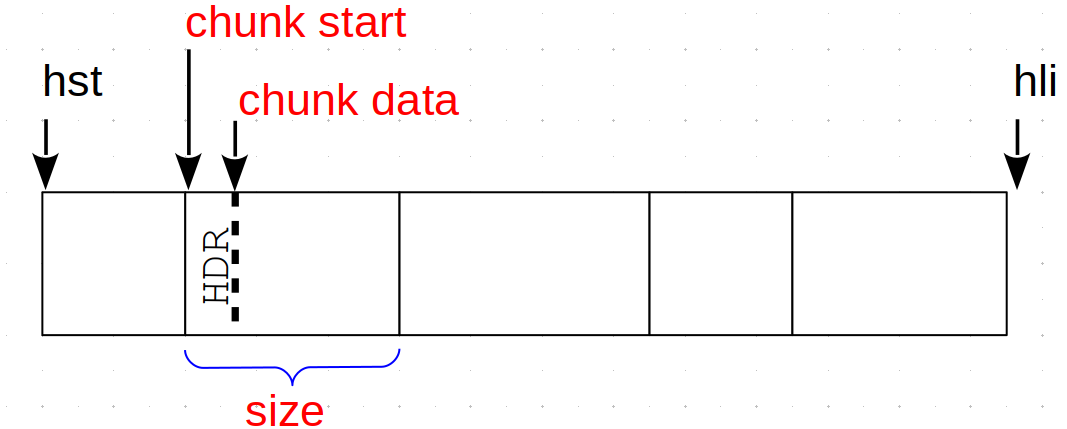
\includegraphics[width=0.8\textwidth]{figures/chunk}
    \caption{Chunk's internals}
    \label{fig:chunkrep}
    \end{center}
\end{figure}

There is a balance to find between the size of information stored in the meta-data and the memory consumption.
More information may lead to faster algorithms, but also reduces the available memory.
Let us present several ways of defining chunk header.

A chunk header storing the full information can be defining using the following C structure:
\begin{lstlisting}[style=cstyle]
typedef struct header
{
  size_t size;
  bool isfree;
  struct header *fpr;
  struct header *fnx;
} header;
\end{lstlisting}
where the field \code{size} stores the size in bytes of the full chunk (including the header), \code{is free} is the flag storing the status of the chunk, and \code{fpr} resp. \code{fnx} are used to implement the list of free chunks (and they are valid only if \code{isfree} is true).

A more compact solution for the header may be obtained if the flag for the chunk's status is stored with the size information. This is possible if the DMA maintains only chunks of even size. Therefore, the least significative bit of the size is always zero and may be used to store the flag on the status of the chunk.
Also, the list of free chunks may be only singly linked, therefore the \code{fpr} field may be eliminated.
The following definition implements this more compact solution:
\begin{lstlisting}[style=cstyle]
typedef struct header
{
  size_t size;			
  struct header *fnx;
} header;
\end{lstlisting}
and it will be used in the next section in the code I've implemented.
Notice that we can get the chunk size by doing a bitwise operation. 
The following chunk in the heap region is obtained by summing the address of the current chunk and the size of the chunk. The following macro-definitions get or set the information of the header defined above.
\begin{lstlisting}[style=cstyle]
// methods to get header information
#define HDR_GET_SIZE(p)     (p->size & (~1))
#define HDR_GET_STATUS(p)   (p->size & 1)
#define HDR_GET_NEXT(p)     ((header*) p + HDR_GET_SIZE(p))
#define HDR_SET_SIZE(p,nh)  p->size = (((nh + 1) >> 1) << 1) & (~HDR_GET_STATUS(p))
#define HDR_SET_STATUS(p)   p->size = p->size | 1
#define HDR_UNSET_STATUS(p) p->size = p->size & (~1)
\end{lstlisting}

The most compact solution is the one storing only an integer (4 bytes) as header. This integer may store the size of the chunk and the flag (as explained above), or the next pointer and the flag (if the addresses of chunks are always even).
The free list is not kept, which means that the DMA has to scan all the chunks to find the free ones and therefore is slower.
The following definition implements this very compact solution:
\begin{lstlisting}[style=cstyle]
typedef int header;
\end{lstlisting}


\subsection{Allocation Algorithms}
One of the important part of \code{malloc} is the way that free chunks are found and allocated. In what follows, we will discuss some policies and algorithms used to perform a dynamic allocation when the free chunks are stored in a list.
Figure~\ref{fig:freelist} illustrates a heap region managed by the DMA with free list.

\begin{figure}[htbp]
    \begin{center}
        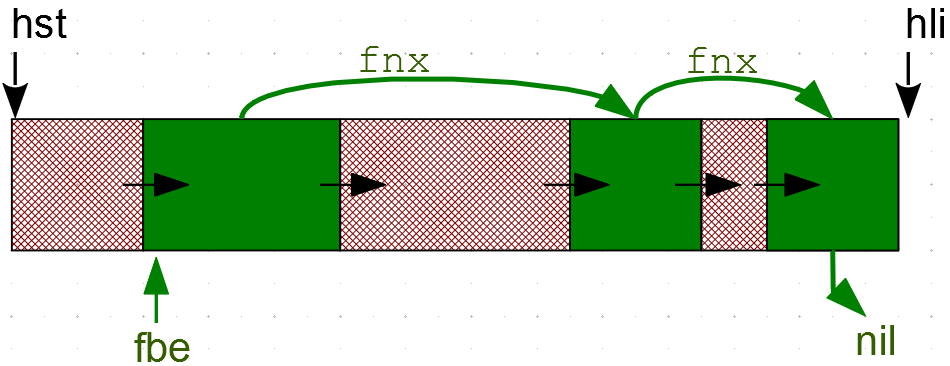
\includegraphics[width=0.8\textwidth]{figures/freelist}
    \caption{Heap with free list in green}
    \label{fig:freelist}
    \end{center}
\end{figure}

%First-fit method
\subsubsection{First-fit method}
The first-fit method allocates the first free chunk in the free list which has sufficient size to satisfy the request. If such a chunk does not exist, there are several choices.
In lazy allocators, a coalescing of neighboring free chunks is done, and then the DMA tries again to find a suitable free chunk.
Otherwise, if the break point does not reached the heap limit, the DMA has the choice to increase the size of the heap region managed using \code{sbrk()}, and then try the allocation again.
If this fails, the allocation also fails.

\begin{figure}[htbp]
    \begin{center}
        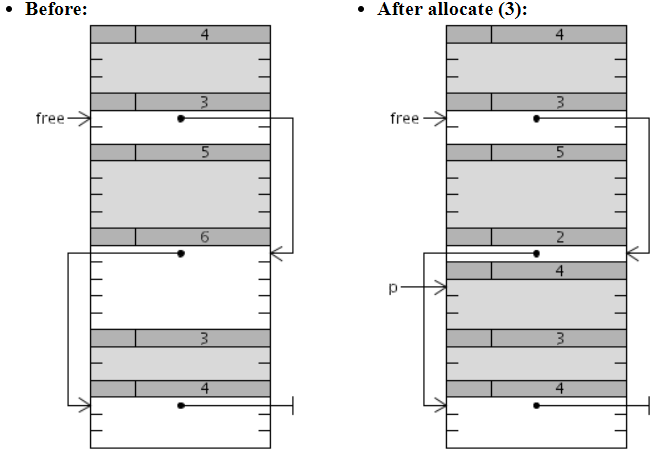
\includegraphics[width=0.8\textwidth]{figures/FF_alg}
    \vspace{-3eX}
    \caption{First fit execution for a request of size 3}
    \label{ff_alg}
    \end{center}
    \vspace{-3eX}
\end{figure}

%first fit algorithm
\begin{algorithm}
\caption{Algorithm for malloc(n)}
\begin{small} 
\begin{algorithmic} 
\REQUIRE $n \geq 0$
\STATE $rsize \leftarrow n + size(header)$  
\STATE Scan free list for first chunk with size $\geq rsize$ 
\IF{chunk not found} 
  \STATE Failure (time for coalescing!) 
\ELSIF{free chunk size is $k \geq rsize + size(header) + 1$} 
   \STATE Split chunk into a free chunk and a busy chunk of size $rsize$
   \STATE Free chunk size $\leftarrow k - rsize$
   \STATE Busy chunk size $\leftarrow rsize$
    \STATE Return pointer to the data part of the Busy chunk 
\ELSE 
    \STATE Unlink chunk from free list 
    \STATE Return pointer to the data part of the chunk 
\ENDIF
\end{algorithmic}
\end{small} 
\end{algorithm}

The main advantage of this method is the fastest search.
The disadvantage, studied in \cite{Knuth73a}, is the localization of the in-use chunks at the start of the heap region.

%best fit algo
\subsubsection{Best-fit method}
The best fit method allocates the free chunk which has the smallest sufficient size.
If such a chunk does not exist, the best fit proceeds like in the failure case of the first-fit method: 
first it tries the coalescing of neighboring free chunks, then it increases the size of the heap region managed.

\begin{figure}[htbp]
    \begin{center}
        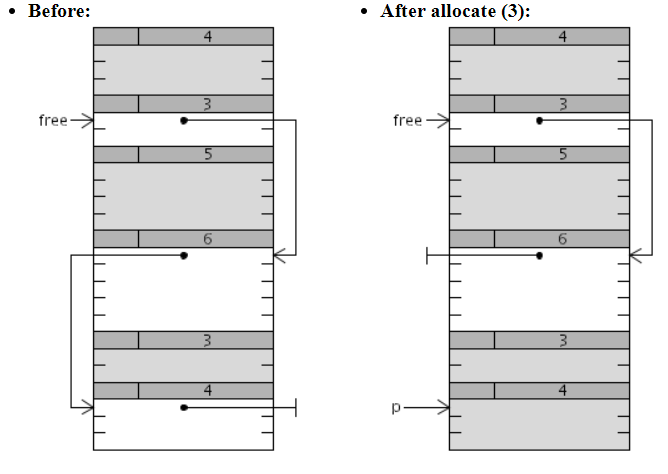
\includegraphics[width=0.8\textwidth]{figures/BF_alg}
    \caption{Best fit execution for a request of size 3}
    \label{bf_alg}
    \end{center}
\end{figure}
%best fit algorithm
\begin{algorithm}
\caption{Algorithm for allocate (n)}
\begin{algorithmic} 
\REQUIRE $n \geq 0$
\REQUIRE $n \geq 0$
\STATE $rsize \leftarrow n + size(header)$  
\STATE Scan free list for for smallest block with size $\geq rsize$ 
\IF{chunk not found} 
  \STATE Failure (time for coalescing!) 
\ELSIF{free chunk size is $k \geq rsize + size(header) + 1$} 
   \STATE Split chunk into a free chunk and a busy chunk of size $rsize$
   \STATE Free chunk size $\leftarrow k - rsize$
   \STATE Busy chunk size $\leftarrow rsize$
    \STATE Return pointer to the data part of the busy chunk 
\ELSE 
    \STATE Unlink chunk from free list 
    \STATE Return pointer to the data part of the chunk 
\ENDIF
\end{algorithmic}
\end{algorithm}


Although best fit minimizes the wastage space, it consumes a lot of time for searching the chunk with smallest size.
 
\subsubsection{Coalescing of free chunks}

Coalescing may be done either at the call of \code{free} (early coalescing allocators) or 
when \code{malloc} does not find a free chunk with enough size (lazy coalescing allocators).

In both cases, the allocator transform the free list by merging in one free chunk two chunks that are neighboring in the heap.
